% !TEX encoding = UTF-8 Unicode
% ------------------------------------------------------------------------------
% Este fichero es parte de la plantilla LaTeX para la realización de Proyectos
% Final de Grado, protegido bajo los términos de la licencia GFDL.
% Para más información, la licencia completa viene incluida en el
% fichero fdl-1.3.tex

% Copyright (C) 2012 SPI-FM. Universidad de Cádiz
% ------------------------------------------------------------------------------


\section{Metodologí­a de desarrollo}

Previamente al desarrollo de la aplicación web, se ha llevado a cabo el de la web pública de la empresa. Para ello, se ha realizado un diseño inicial de forma orientativa para su posterior desarrollo y pruebas de funcionamiento en diferentes dispositivos. Una vez finalizada, y al poder ser usada independientemente, se ha puesto en producción mientras se implementaba el área de cliente, la parte principal en la que se centrará el proyecto.
\\

Para el desarrollo de la mencionada aplicación web se ha usado un modelo incremental e iterativo. Primeramente se realizó un análisis de la aplicación en general y herramientas a utilizar para su desarrollo. A partir de ahí, se inicia el proceso de implementación del producto divido en varios ciclos, en los cuales se han ido añadiendo distintas funciones a la aplicación, obteniendo así una versión más completa al final de cada una de las fases. En cada una de ellas se analiza, diseña, implementa y prueba estas funcionalidades a añadir.
\\

A continuación, se describirá las tareas realizadas en cada uno de estos ciclos:

\subsection{Primer Ciclo}

Primero de todo, se ha estructurado la implementación del proyecto en distintos módulos. Una vez hecho esto, se ha configurado el servidor de aplicaciones y definido los distintos tipos de usuarios del sistema, implementando seguidamente el registro e identificación de usuarios, con manejo de sesiones y de errores.
\\

A su vez, se ha realizado el diseño general de la interfaz del software, que se ha aplicado a las pantallas de esta fase del desarrollo, como registro de usuario, inicio de sesión o la página de inicio una vez realizado el login, teniendo en cuenta que existen diferentes vistas de la interfaz dependiendo del tipo de usuario. \\
Esta será multilenguaje, dando opción al usuario a elegir su lenguaje por defecto seleccionándolo en el menú desplegable para tal efecto.

\subsection{Segundo Ciclo}

En este segundo ciclo se ha implementado todo lo relacionado con la gestión de usuarios: vista y edición del perfil de los usuarios registrados, gestión de los mismos por parte de administradores, gestión de administradores por el super-administrador, comunicación entre todo tipo de usuario, histórico de acciones en el sistema, etc.

\subsection{Tercer Ciclo}

Este ciclo comprende la principal funcionalidad del sistema, la gestión de actividades y citas. Se ha desarrollado la creación de servicios, actividades, citas, etc., junto a consulta de los mismos, edición, altas, bajas... Siempre desde una interfaz intuitiva que incluye un calendario donde ver toda la actividad del usuario. \\

Es la parte más compleja e interesante del producto, ya que cumple el principal requisito funcional por el cual se ha realizado este proyecto.

\subsection{Cuarto Ciclo}

En este último ciclo de implementación se han añadido las funcionalidades restantes para la finalización del producto, como notificaciones, contacto o contenido de la página de inicio, por ejemplo. 


\subsection{Quinto Ciclo: Pruebas}

Finalmente, se han realizado las pruebas pertinentes del software y se ha procedido a subsanar los errores encontrados y llevar a cabo pequeñas mejoras. Aclarar que en cada ciclo se han realizado pruebas manuales de la parte correspondiente, por lo que esta fase final de pruebas se ha realizado sin mucha incidencia.


\section{Planificación del proyecto}

En la figura \ref{fig:diagrama-gantt} se muestra la planificación temporal del desarrollo del proyecto a través de un diagrama de Gantt. En él, se muestran las tareas realizadas divididas por bloques y el tiempo estimado de realización para cada una de ellas. \\

\begin{figure}
\centering
  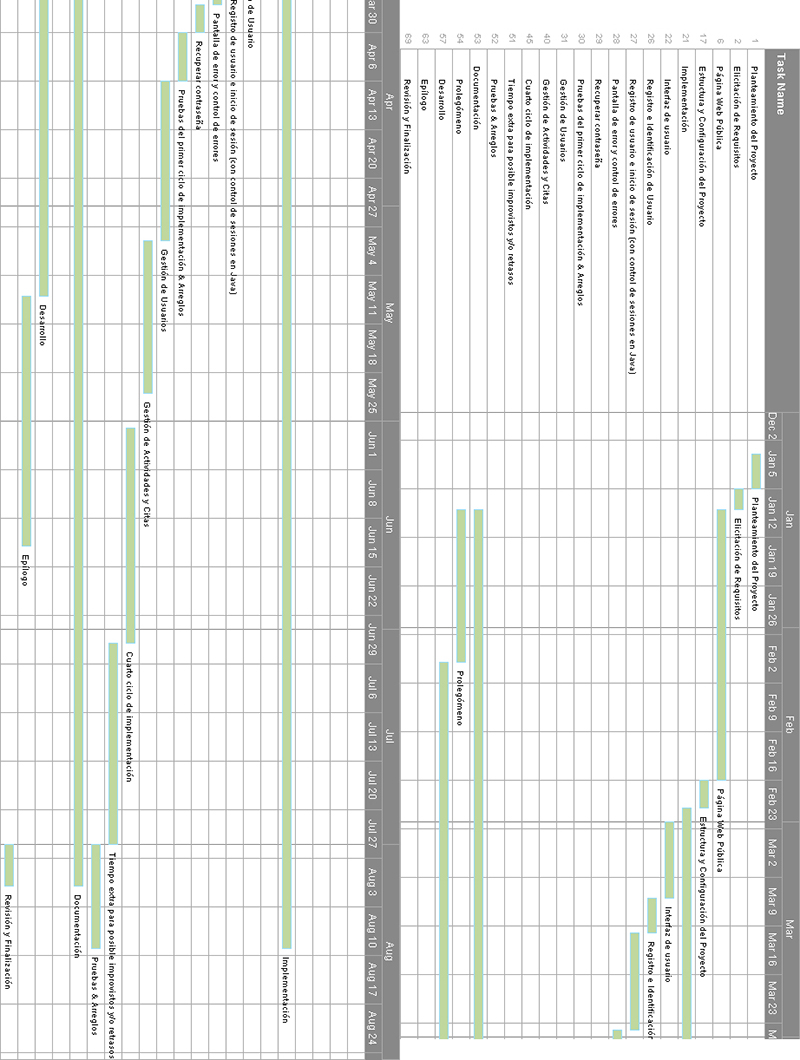
\includegraphics[scale=.50]{img/diagrama-Gantt.jpg}
  \caption{\textit{Planificación temporal a través de diagrama de Gantt.}}
  \label{fig:diagrama-gantt}
\end{figure}

Observamos que desde el inicio del proyecto hasta su finalización transcurrirán 7 meses aproximadamente, divididos en varios bloques bien diferenciados, como son: \textit{Planteamiento y Planificación, Elicitación de Requisitos, Página Web Pública, Estructura y Configuración del Proyecto} e \textit{Implementación}.\\

A pesar de que el periodo empleado desde que se inició del proyecto hasta su finalización ha sido bastante mayor al estimado, se puede afirmar que el tiempo real que se ha dedicado al proyecto se asemeja a los 7 meses planificados. Esta estimación se realiza suponiendo que la disponibilidad para llevarla a cabo es casi total; sin embargo, en la práctica, el desarrollo del proyecto se ha compaginado con otras tareas, como estar empleado durante la mayor parte del tiempo, realización de proyectos por cuenta propia, voluntariados, etc. 


\section{Organización}

Respecto al desarrollo de la aplicación, he sido el único desarrollador, a la vez de testeador. La tutora del proyecto ha sido Lorena Gutiérrez Madroñal, guiándome en su proceso y asegurándose que cumplía los requisitos suficientes para que sea un proyecto completo. 
\\

En cuanto al cliente, los dos socios de \textsl{CoreSport} con los que he mantenido la comunicación durante el proceso de desarrollo, y posterior a este, han sido Ángel Soriano y Cristina Saucedo. Ellos serán los administradores del sistema, con opción de añadir algunos de los trabajadores restantes en el centro, como monitores de las clases, responsables de servicios externos o recepcionista. 
\\

El resto de usuarios del software serán los clientes de la empresa, que serán los usuarios finales del producto mediante previo registro.
\\

El hardware utilizado para el desarrollo ha sido el propio ordenador portátil del alumno, un MacBook Pro, sirviendo así de entorno de programación y pruebas mediante el uso del siguiente software: 

\begin{itemize}
\item \textbf{macOS Yosemite (10.10), El Capitán (10.11) y Sierra (10.12)} como sistemas operativos a lo largo de todo el desarrollo.
\item \textbf{Glassfish} como servidor de aplicaciones local.
\item \textbf{NetBeans} como entorno de desarrollo.
\item \textbf{pgAdmin} como gestor y administrador de bases de datos, usando \textbf{PostgreSQL} como sistema de gestión.
\item \textbf{Git} como sistema de control de versiones.
\item \textbf{TeXShop} como editor de textos para la documentación en \textbf{LaTeX}.
\end{itemize}


\section{Costes}

Durante el desarrollo de este proyecto no se ha realizado ningún coste extra al trabajo de desarrollo por parte del alumno y los gastos comunes que pueden ocasionar, como desplazamiento para entrevistas, luz, etc. Por lo que se calculará el total de costes en función al tiempo estimado de desarrollo del proyecto por parte de un ingeniero informático.\\

Según la estimación temporal realizada anteriormente, la realización de la totalidad del proyecto comprendería un periodo de 7 meses. De acuerdo a lo establecido en el \textit{Convenio colectivo del sector de empresas de ingeniería y oficinas de estudios técnicos}, publicado en el \textit{BOE (Boletín Oficial del Estado)} el miércoles 18 de enero de 2017 \cite{BOE18ene17}, el salario pactado para \textit{Nivel 1. Licenciados y titulados 2.º y 3.er ciclo universitario y Analista} es de 1.687,02€ mensuales (x 14 meses) o, lo que es lo mismo, 1968,19€ mensuales si se divide en 12 meses. Por tanto, la estimación del coste total del proyecto sería de 1968,19€ x 7 meses = 13777,33€.


\section{Riesgos}

Primeramente, tendremos en cuenta el riesgo del hardware. No sabemos cuál va a ser la vida de nuestro equipo en el que estamos desarrollando una aplicación, por lo que siempre debemos tener una copia de nuestro código para evitar posibles pérdidas de datos, ya sea por avería o rotura. Para ello, se ha utilizado \textit{Subversion}, un sistema de control de versiones que puede ser usado desde nuestro entorno de programación \textit{Netbeans}, brindando una herramienta esencial y sencilla de usar. Tendremos así nuestra implementación en un lugar seguro, además de beneficiarnos de las opciones que un control de versiones ofrece.
\\

Uno de los posibles riesgos que no podremos controlar es el cambio de requisitos durante el desarrollo del proyecto. Es común que los clientes cambien o añadan funcionalidades al sistema cuando van viendo algunos resultados, probando prototipos o simplemente puntos que se les haya pasado anteriormente. \\
Estos cambios conllevarán un tiempo extra en el desarrollo del producto. De aquí la importancia de la fase de elicitación de requisitos y la comunicación con el cliente, para tratar de obtener unos requisitos bien definidos desde el principio y evitar así posibles cambios o nuevas funciones a añadir.
\\

Otro riesgo potencial en la implementación del software es la actualización de las versiones de la tecnología que estemos usando. Es decir, cuando usamos librerías, frameworks, APIs, etc., estamos expuestos a que estos se actualicen, o incluso dejen de tener soporte. Al ser, de nuevo, un factor externo al desarrollo, no se podrán tomar grandes medidas de prevención, pero sí se puede mejorar con una buena decisión respecto qué tecnologías usar en nuestro desarrollo. \\
En el desarrollo del software, la inmensa mayoría de las veces existirán diversas formas de conseguir un objetivo. De aquí que tengamos la opción de decidir qué lenguaje de programación, librerías, frameworks, APIs... usar. Aun así, si nos vemos en el hecho de tener que realizar cambios en alguna de ellos durante o después del desarrollo, el impacto no debería ser muy grande con una implementación limpia y bien construida. 
\\

Un ejemplo clásico de riesgo podría ser la estimación del tiempo de desarrollo del proyecto. Es común que este sea menor al tiempo real de desarrollo y, como consecuencia, existe un incremento de recursos: el tiempo de entrega del proyecto, gastos extras -ya sea para el cliente o el equipo de desarrollo- o pérdida de beneficios para negocios que no obtienen su software a tiempo. En este caso, un retraso en la estimación del tiempo no traería grandes consecuencias, los usuarios y administradores del centro seguirán llevando la misma rutina de gestión hasta que el producto esté listo para pasar a fase de producción.
\\

Una vez el producto esté en producción, su rendimiento dependerá de un servidor contratado, por lo que es un riesgo externo a tener en cuenta. Si el servidor bajo el que la aplicación esté funcionando falla, no se tendrá acceso a la misma. Este es un riesgo que no podemos controlar, y se confía en que la empresa encargada del mismo tome medidas de seguridad suficientes para que, en el caso de fallo, el servicio no sufra caída alguna. 


